\documentclass{article}
\usepackage{listings}
\usepackage{color}
\usepackage{graphicx} 
\usepackage{float}
\definecolor{codegreen}{rgb}{0,0.6,0}
\definecolor{codegray}{rgb}{0.5,0.5,0.5}
\definecolor{codepurple}{rgb}{0.58,0,0.82}

\definecolor{backcolour}{rgb}{0.95,0.95,0.92}
\lstdefinestyle{mystyle}{
    backgroundcolor=\color{backcolour},   
    commentstyle=\color{codegreen},
    keywordstyle=\color{magenta},
    numberstyle=\tiny\color{codegray},
    stringstyle=\color{codepurple},
    basicstyle=\ttfamily\footnotesize,
    breakatwhitespace=false,         
    breaklines=true,                 
    captionpos=b,                    
    keepspaces=true,                 
    numbers=left,                    
    numbersep=5pt,                  
    showspaces=false,                
    showstringspaces=false,
    showtabs=false,                  
    tabsize=2
}

\lstset{style=mystyle}

\title{Muestreo de Señal PWM}
\author{Oscar Ivan Moreno Gutierrez}
\date{\today}

\begin{document}

\maketitle

\section{Descripción}
Este proyecto se centra en realizar medidas sobre dos señales que se obtienen al filtrar una señal PWM generada con el dsPIC. Las medidas que se realizan incluyen el valor máximo, el valor medio y el valor eficaz de las señales. La información obtenida de ambas señales se muestra en una pantalla LCD. Además, se crea un filtro digital utilizando la herramienta de MATLAB para procesar las señales.
\section{Archivos y Directorios}
\begin{itemize}
\item \texttt{main.c}: Este es el archivo principal de mi proyecto. Incluye la función 
\item \texttt{pintar\_lcd.h}: Este archivo se utiliza para funciones relacionadas con la visualización LCD.
\end{itemize}

\section{Funciones}
\begin{itemize}
\item \texttt{EJEMPLO}: bla bla bla
\end{itemize}

\section{Procedimiento}
Empezamos con la creacion de las funciones basicas del dsPIC utilizando un SSCP para una salida PWM, Cumpliendo el con el esquema proporcionado (Figura \ref{fig:esquema}).

\begin{figure}[H]
    \centering
    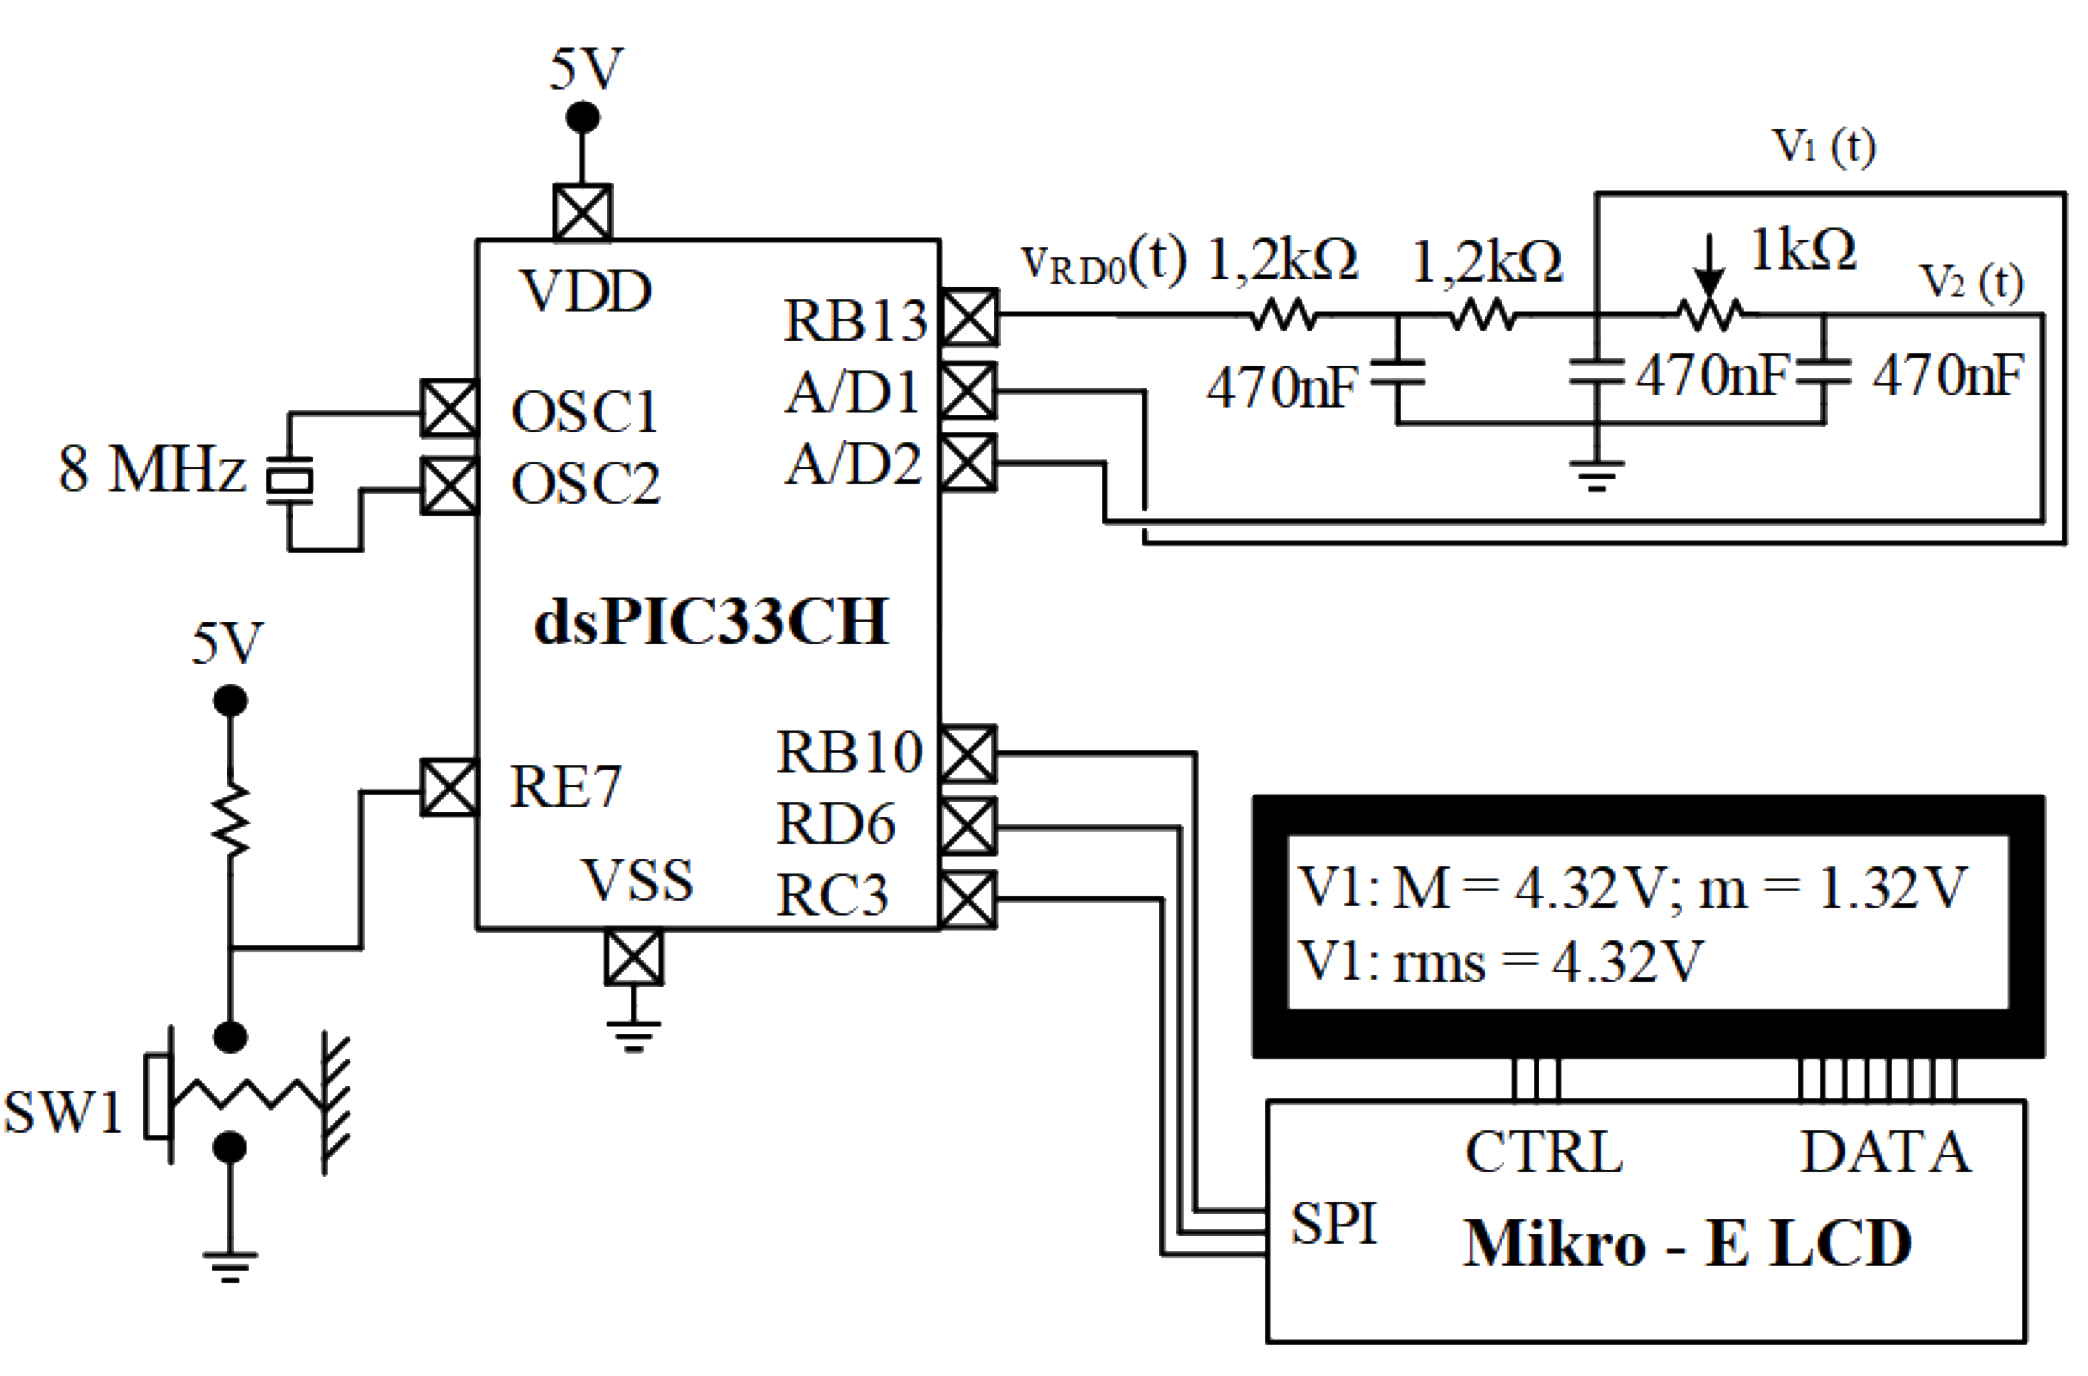
\includegraphics[width=0.5\textwidth]{images/esquema_og.png} % Replace with the path to your image
    \caption{Esquema del proyecto}
    \label{fig:esquema}
\end{figure}
La salida PWM sale por el RB13 y se conecta con un filtro proporcionado por el profesor.Donde se obtienen las señales senoidal y triangular.
Una mejora seria la implementacion de manipular el ciclo de trabajo con un modulo ADC. Utilizando un potenciometro para manipular el ciclo de trabajo de la señal PWM.

Posteriormente, realizo las medidas de las señales, los visualize en un osciloscopio. Como se muestra en la Figura \ref{fig:osciloscopio}.
\begin{figure}[H]
    \centering
    %%\includegraphics[width=0.5\textwidth]{path/to/your/image} % Replace with the path to your image
    \caption{Caption of the figure}
    \label{fig:osciloscopio}
\end{figure}

\section{Código}
\begin{lstlisting}[language=C]
    Hello world
\end{lstlisting}

\section{Cómo ejecutar}
Proporcione instrucciones sobre cómo compilar y ejecutar su proyecto.

\end{document}